\section{Finite terms}

Let $\Upsilon$ be a nonempty collection of node variables and $X$ a collection of edge variables. $\mathcal{C}$ is a collection of constant terms, which will be specified later. We have at our disposal an unspecified collection of names, in case we need them. All these collections are disjoint sets. 

The collection $\mathcal{C}$ contains at least four terms: $0$, $1$, $\displaystyle \bar{1}$ and $T$. The last one is called the terminator. 



\begin{definition}
Any finite term is obtained after a finite number of applications of the following rules:
\begin{enumerate}
\item[-] if $x \in X$ is an edge variable then $x$ is a term. $Nodevar(x)=\emptyset$ and $Edgevar(x)=\left\{ x \right\}$.
\item[-] if $x,y$ are terms and $a \in \Upsilon$ is a node variable then $\displaystyle a^{x}y$ and $\displaystyle \bar{a}^{x}y$  are terms. 
$$Nodevar\left( a^{x} y \right) = Nodevar\left( \bar{a}^{x} y \right) =  \left\{ a \right\} \cup Nodevar(x) \cup Nodevar(y)$$
$$Edgevar\left( a^{x} y \right) = Edgevarvar\left( \bar{a}^{x} y \right) = Edgevar(x) \cup Edgevar(y)$$
\item[-] any constant term is a term. 
\end{enumerate}

The arity of a term $x$ is the number of elements of $Edgevar(x)$. The terminator has arity 1, $0$ and $1$ have arity 2.

A node variable $a \in \Upsilon$ is fresh for a term $x$ if $\displaystyle a \not \in Nodevar(x)$. An edge variable $y \in X$ is fresh for a term  $x$  if 
$\displaystyle y \not \in Edgevar(x)$.

Two terms are equal "$x=y$" if they are identical up to alpha renaming of their node and edge variables. 
\label{defterms}
\end{definition}



We represent terms by their syntactic trees. A syntactic tree is a particular case of an oriented ribbon graph, where we assume that the edges of the syntactic tree are oriented from the leaves to the root and that any node of the syntactic tree has only one output edge and the order of the other edges comes from the clockwise orientation, starting from the output edge. We do not distinguish between terms and their graph representation. 





The following convention is used: we are free to define a term by giving it a name (which should not be a node or edge variable). Graphically a defined term appears as a node with the name of the term and a collection of half edges. If the term has arity $n$ then as a node in an oriented ribbon graph it will have $n+1$ half edges (except for the terminator), which can be uniquely identified by their  appearance in the clockwise order. The node variables of the term appear as decorations of the node. The input half edges are decorated with terms. (Some times we shall use another color, for example red, for the decorations of the leaves. Other times we shall just number the leaves, in the right order.) The root is left without any decoration (other than the terminator, perhaps). 

Whenever we draw syntactic trees, the root will appear at the left of the figure. In this way the orientations of the edges can be deduced from the rules from the clockwise order on the page, the position of the root and the color or names of the nodes. 

\vspace{.5cm} 
\centerline{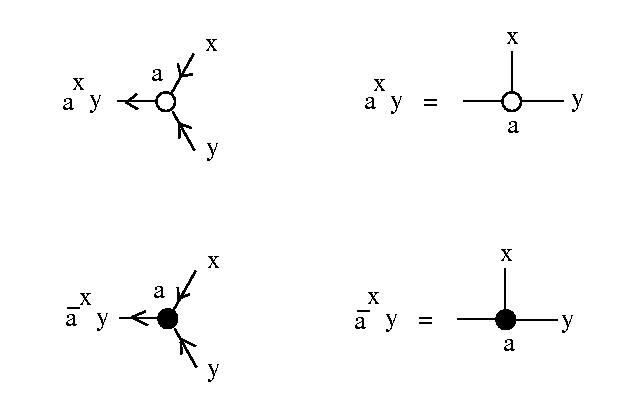
\includegraphics[width=80mm]{jpg/shuffle_00.jpg}} \vspace{.5cm} 

If $a \in \Upsilon$ and $x , y$ are terms then the term $\displaystyle a^{x}y$ appears as a white (or empty) circle, decorated with $a$, and the term $\displaystyle a^{x}y$ appears as a white (or empty) circle, decorated with $a$. 



A forrest of trees, with only one root which is not decorated by a terminator, counts for us as a term. 

The terminator is seen as a decoration of a root of a syntactic tree. The convention is to ignore any tree with the root decorated with a terminator. We need terminators only for technical purposes, like the need to be able to describe rewrites of the constants $0$ and $1$, or to be able to mark some terms for erasure, or for an implementation of a garbage collection algorithm, if needed. For this article the terminator is one of the mild inconveniences due to the fact that written articles are not programs, but any program which implements what is described in the article has to contain a terminator, which is moreover easy to build. On the other side, as articles, less rigorous as programs, are targeted for a human audience,  the concept of a terminator is very easy to grasp. 


 \vspace{.5cm}



Further is a list of terms which are going to be important in the exposition. 



\begin{definition}
If $a \in \Upsilon$ is a node variable and $b$ a binary term (i.e. it has arity 2) then $\displaystyle a-b$ is the term: 

\vspace{.5cm} 
\centerline{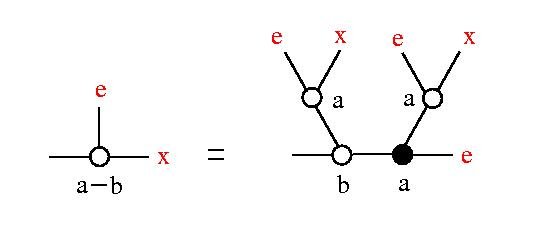
\includegraphics[width=80mm]{jpg/a-b.jpg}} \vspace{.5cm} 


If $a$ and $b$ are binary terms then $\displaystyle ab$ is the term: 

\vspace{.5cm} 
\centerline{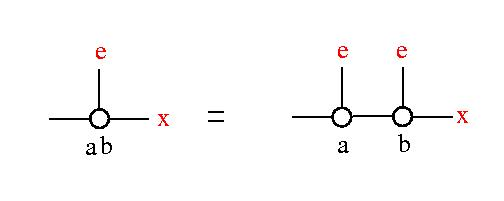
\includegraphics[width=70mm]{jpg/ab.jpg}} \vspace{.5cm} 

The constant terms $0$, $1$ and $\displaystyle \bar{1}$ have arity 2 and are defined via the terminator, as: 

\vspace{.5cm} 
\centerline{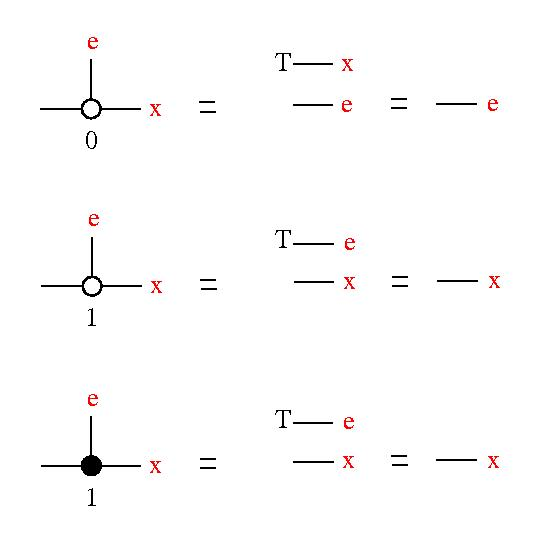
\includegraphics[width=70mm]{jpg/0.jpg}} \vspace{.5cm} 

\label{ddifprod}
\end{definition}
